% Written by Daina Chiba (daina.chiba@gmail.com).
% It was mostly copied from two poster style files:
% beamerthemeI6pd2.sty written by
%	 	Philippe Dreuw <dreuw@cs.rwth-aachen.de> and 
% 		Thomas Deselaers <deselaers@cs.rwth-aachen.de>
% and beamerthemeconfposter.sty written by
%     Nathaniel Johnston (nathaniel@nathanieljohnston.com)
%		http://www.nathanieljohnston.com/2009/08/latex-poster-template/
% 
% Modified for UvA by
% Maarten de Rijke, April 2014
%
%---------------------------------------------------------------------------------------------------% 
% Preamble
% ---------------------------------------------------------------------------------------------------% 
\documentclass[final]{beamer}
\usepackage[orientation=landscape,size=a0,scale=1.2,debug]{beamerposter}
\mode<presentation>{\usetheme{UvAPoster}}
\usepackage[english]{babel}
\usepackage[latin1]{inputenc}
\usepackage[T1]{fontenc}
\usepackage{amsmath,amsthm, amssymb, latexsym}
\usepackage{exscale}
\usepackage{caption}

\usepackage{array,booktabs,tabularx}
\newcolumntype{Z}{>{\centering\arraybackslash}X} % centered tabularx columns

% comment 
\newcommand{\comment}[1]{}

% (relative) path to the figures
\graphicspath{{figs/}}

\newlength{\columnheight}
\setlength{\columnheight}{105cm}
\newlength{\sepwid}
\newlength{\onecolwid}
\newlength{\twocolwid}
\newlength{\threecolwid}
\setlength{\sepwid}{0.024\paperwidth}
\setlength{\onecolwid}{0.24\paperwidth}
\setlength{\twocolwid}{0.4\paperwidth}
\setlength{\threecolwid}{0.19\paperwidth}

\setbeamertemplate{bibliography item}{\insertbiblabel}
\setbeamertemplate{bibliography entry article}{}
\setbeamertemplate{bibliography entry title}{}
\setbeamertemplate{bibliography entry location}{}
\setbeamertemplate{bibliography entry note}{}
\setbeamertemplate{bibliography entry year}{}
\setbeamertemplate{caption}[numbered]

% ---------------------------------------------------------------------------------------------------% 
% Title, author, date, etc.
% ---------------------------------------------------------------------------------------------------% 
\title{\huge Are Neural Click Models Pointwise IPS Rankers?}
\author{Philipp Hager\inst{1} \and Maarten de Rijke\inst{1} \and Onno Zoeter\inst{2}}
\institute[shortinst]{\inst{1} University of Amsterdam \inst{2} Booking.com}
\date[Sep. 2022]{September, 2022}
%%% Put the name of conference here.
\def\conference{CONSEQUENCES+REVEAL Workshop at RecSys '22} 
%%% Put your e-mail address here.
\def\yourEmail{p.k.hager@uva.nl}

% ---------------------------------------------------------------------------------------------------% 
% Contents
% ---------------------------------------------------------------------------------------------------% 
\begin{document}
\begin{frame}[t]
	\begin{columns}[t]
	% -----------------------------------------------------------
	% Start the first column
	% -----------------------------------------------------------
	\begin{column}{\onecolwid}
		
	% -----------------------------------------------------------
	% 1-0
	% -----------------------------------------------------------
	\begin{block}{Introduction}

		Inverse-propensity scoring (IPS) and click models (CM) are prevalent methods for learning rankers from position-biased click data:
		\vspace{1ex}
		\begin{itemize}
			\item {\bf IPS methods}: Assume position bias is known, typically use document features and optimize point-/pair-/listwise rankings.
			\item {\bf Click models}: Infer position bias, typically treat each document separately and make pointwise relevance estimations.
		\end{itemize}

		\vspace{1ex}

		Is a neural click model leveraging document features equivalent to a pointwise IPS ranker when both use the same position bias estimation?

		\vspace{1ex}

		\begin{itemize}
			\item We compare both approaches theoretically.
			\item We perform an empirical comparison on semi-synthetic click data.
		\end{itemize}

	\end{block}

	\vspace{1ex}

	% -----------------------------------------------------------
	% 1-1
	% -----------------------------------------------------------
	\begin{block}{Methods}

		\textbf{Neural click model:} Predicts biased user clicks. Document relevance $\hat{y}_d$ and position bias $\hat{o}_k$ are latent parameters inferred by minimizing binary cross-entropy between predicted and observed clicks~\cite{Yan2022TwoTowers}:
		\vspace{1ex}
		%
		\begin{equation*}
			\begin{split}
			\mathcal{L}_{\text{pbm}}(\hat{y}, \hat{o}) &= - \sum_{(d, k) \in D} c_{d,k} \cdot \log(\hat{y}_{d} \cdot \hat{o}_{k}) + (1 - c_{d,k}) \cdot \log(1 - \hat{y}_{d} \cdot \hat{o}_{k}).
			\end{split}
		\end{equation*}
		%

		\vspace{1ex}
		
		\textbf{Pointwise IPS:} Directly predicts document relevance $\hat{y}_d$ by weighting clicks inversely to the probability of being observed by the user~\cite{Saito2020PointwiseIPS}:
		\vspace{1ex}
		%
		\begin{equation*}
			\begin{split}
			\mathcal{L}_{\text{ips}}(\hat{y}, \hat{o}) = - \sum_{(d,k) \in D} \frac{c_{d,k}}{\hat{o}_k} \cdot \log(\hat{y}_{d}) + (1 - \frac{c_{d,k}}{\hat{o}_k}) \cdot \log(1 - \hat{y}_{d}).
			\end{split}
		\end{equation*}
		%

	\end{block}

	\vspace{1ex}
	
	% -----------------------------------------------------------
	% 1-2
	% -----------------------------------------------------------
	\begin{alertblock}{Comparing unbiasedness}
		\vspace{1ex}

		\begin{itemize}
			\item \textbf{IPS}: Saito et al. show that the pointwise IPS estimator is unbiased when correctly estimating position bias~\cite{Saito2020PointwiseIPS}.
			\item \textbf{CM with joint parameter inference}: Oosterhuis shows that click models jointly inferring bias and relevance are not always consistent estimators of document relevance~\cite{Oosterhuis2022ULTRLimits}.
			\item \textbf{CM only inferring relevance}: \alert{We show that neural click models optimize for unbiased document relevance when, similar to IPS, given access to the true position bias}: $\hat{y} = \frac{o y}{\hat{o}}$.
		\end{itemize}

		\vspace{1ex}

		\begin{figure}[h]
			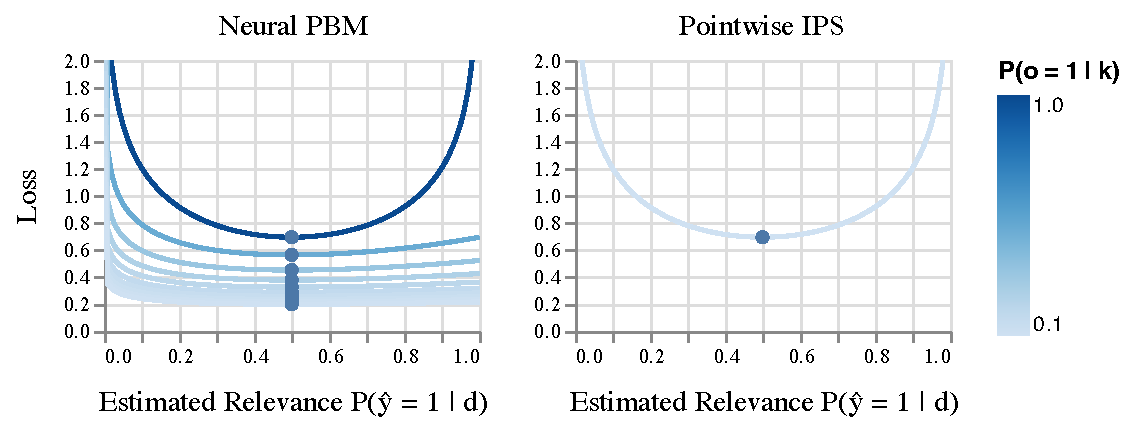
\includegraphics[width=1.\textwidth]{loss.pdf}
			\caption{The loss for a document of relevance $y_d = 0.5$ under varying degrees of position bias. Both methods have their minima at the true relevance, but the magnitude of the click model loss decreases with an increase in bias.}
		\end{figure}

	\end{alertblock}

\end{column}

    % -----------------------------------------------------------
    % Start the second column
    % -----------------------------------------------------------
    \begin{column}{\twocolwid}
	% -----------------------------------------------------------
	% 2-0
	% -----------------------------------------------------------
	\begin{block}{Experimental results}
		
		{\bf RQ:} Given the true position bias, do both approaches perform equally in an empirical comparison?

		\vspace{1ex}

		\begin{figure}[h]
			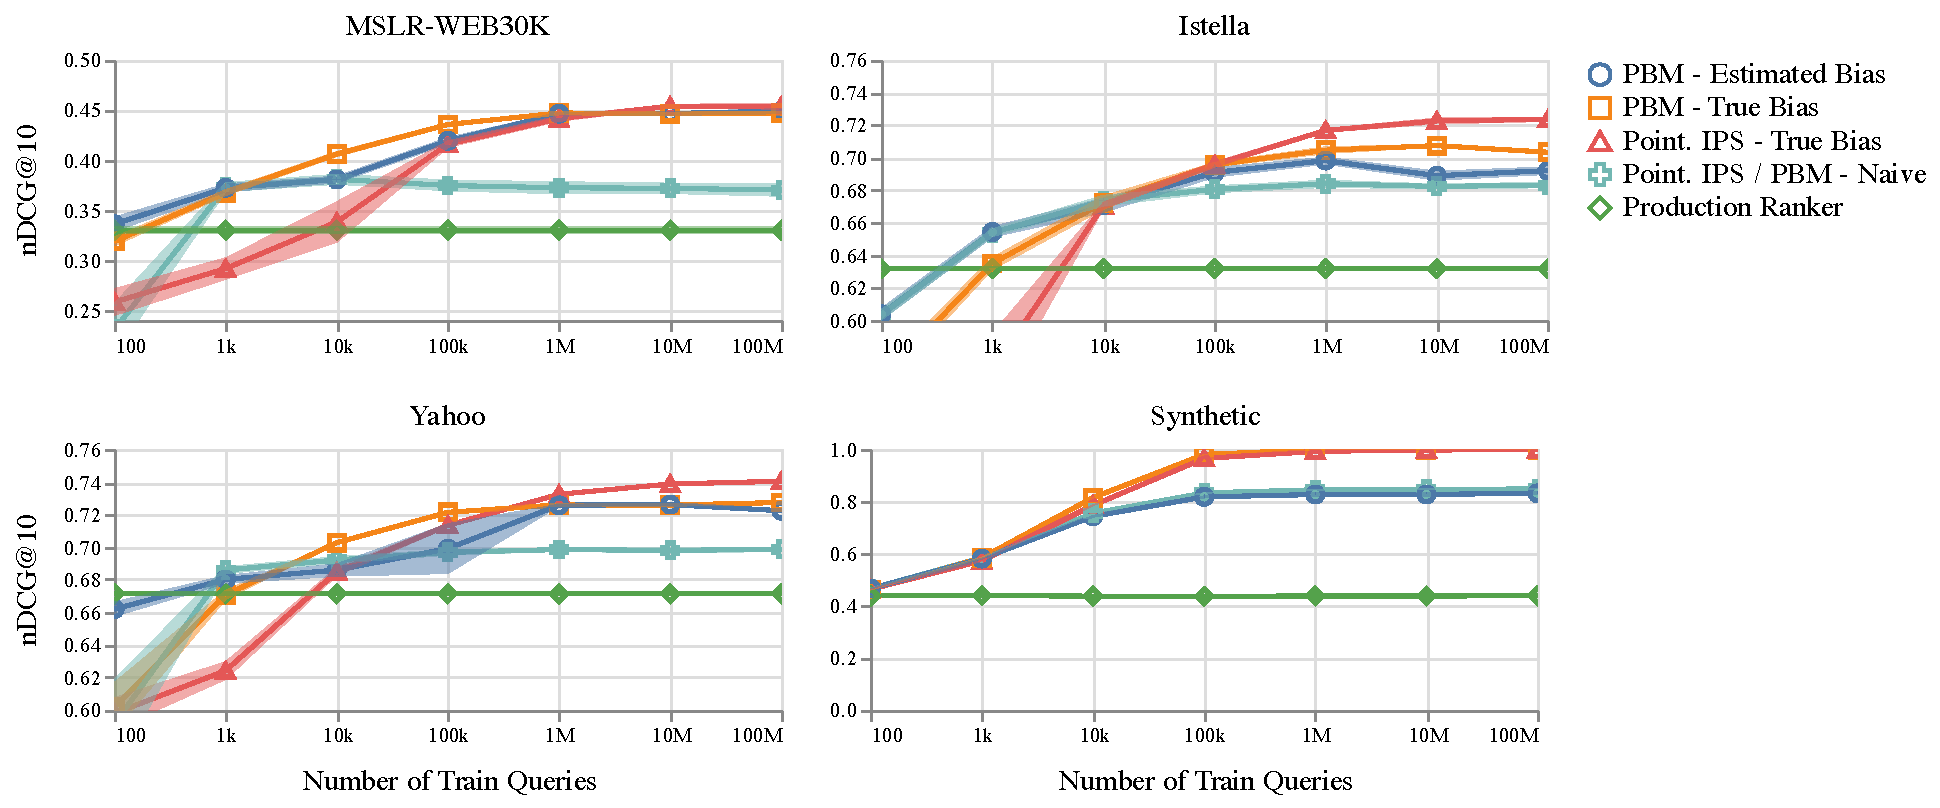
\includegraphics[width=1.\textwidth]{results}
			\caption{Test performance on three large-scale LTR datasets and one fully synthetic dataset after training on up to 100M simulated queries. The simulated user behavior follows the position-based model~\cite{Craswell2008Cascade}. Results are averaged over ten independent experimental runs.}
			\label{fig:results}
		\end{figure}
		
		\vskip1ex

		\begin{itemize}
			\item \textbf{PBM - Estimated Bias}: A neural click model jointly estimating position bias and relevance performs better than a naive baseline that does not compensate for position bias on Yahoo and MSLR-WEB30K.
			\item \textbf{PBM - True Bias}: A neural click model with access to the true position bias has reduced variance and improved performance over the naive baseline on all datasets.
			\item \textbf{IPS - True Bias}: \alert{Pointwise IPS outperforms the neural click model significantly on Istella and Yahoo}.
		\end{itemize}

	\end{block}

	\vspace{2ex}

	% -----------------------------------------------------------
	% 2-1
	% -----------------------------------------------------------
	\begin{block}{Is the neural click model biased?}

		{\bf RQ:} Items at lower position contribute less to the click model's loss, does generalizing over features introduce bias?

		\vspace{1ex}

		\begin{figure}[h]
			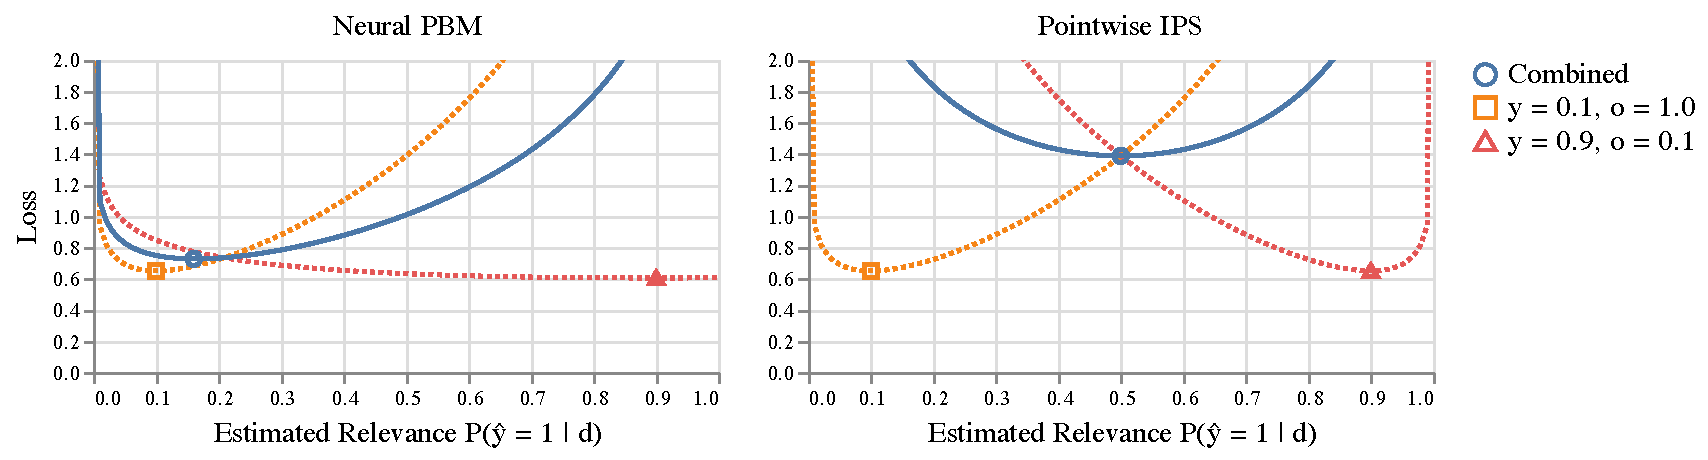
\includegraphics[width=\textwidth]{loss_bias.pdf}
			\caption{Visualizing loss and estimated relevance for an irrelevant document displayed at a high rank (orange square) and a relevant document displayed at a low rank (red triangle). The solid blue line shows the combined loss of both documents.}
  			\label{fig:loss_bias}
		\end{figure}
		
		\vskip1ex
	
		\begin{itemize}
			\item Both approaches converge to the unbiased document relevance when computing the loss for each item separately (dotted lines).
			\item IPS converges to the average relevance of both documents when optimizing the combined loss for both documents (solid line).
			\item \alert{The neural click model converges to a joint document relevance for both documents that is biased towards the item with the higher examination probability}.
		\end{itemize}
	
	\end{block}

\end{column}

% -----------------------------------------------------------
% Start the third column
% -----------------------------------------------------------
\begin{column}{\onecolwid}
	
	% -----------------------------------------------------------
	% 3-0
	% -----------------------------------------------------------
	\begin{block}{Experiments on neural click model bias}
		{\bf We run three additional experiments:}

		\vskip1ex

		\begin{itemize}
			\item {\bf Independent features}: When documents share no features (one-hot encoded documents), the empirical performance of IPS and the neural click model is equivalent (Synthetic in Figure~\ref{fig:results}).
			\item {\bf Feature collisions}: Gradually forcing random documents to share feature vectors leads to a stronger performance drop for the neural click model.
			\item {\bf Position bias recovery}: When simulating increasing levels of position bias, we find that IPS can recover from strong position bias, while the neural click model increasingly deteriorates in performance even if the true position bias is known.
		\end{itemize}

	\end{block}

	\vspace{2ex}

	% -----------------------------------------------------------
	% 3-1
	% -----------------------------------------------------------
	\begin{alertblock}{Conclusion}
		\vskip1ex

		\begin{itemize}
			\item We show that both approaches optimize for unbiased document relevance if the true position bias is known and relevance is estimated separately per query-document pair.
			\item We find the neural click model to be affected by position bias when learning from shared, sometimes conflicting, features instead of estimating each document's relevance separately.
		\end{itemize}

	\end{alertblock}

	\vspace{2ex}

	% -----------------------------------------------------------
	% 3-2
	% -----------------------------------------------------------
	\begin{block}{Selected references}
		\bibliographystyle{acm}
		\bibliography{references}
	\end{block}

	\vspace{2ex}

	\begin{figure}[h]
		
\includegraphics[width=.3\textwidth]{qr}
		\caption*{Scan to read the paper}
	\end{figure}

\end{column}
\end{columns}
\end{frame}
\end{document}
